\section{Clustering}

Clustering is a classification method in unsupervised learning, which we divide data into groups to capture the natural structure of the data. In this section of the report, we are going to cluster the sparm data using both Gaussian Mixture Model (GMM) and hierarchical clustering. In the hierarchical clustering, the cut-off is set at the same number of clusters as astimated by the GMM. Also, the comparision of those two methods will be mentioned afterward.

\subsection{Gaussian Mixture Model}
We validate the number of clusters for Gaussian Mixture Model based on the EM algorithm using cross-validation.Apart from the cross-validation the optimal number of clusters are sometimes derived by penalizing model complexity based on the Bayseian Information Criteria (BIC) or Akaike's Information Criteria (AIC).


%kommentar
\begin{figure}[!ht]
	\centering
	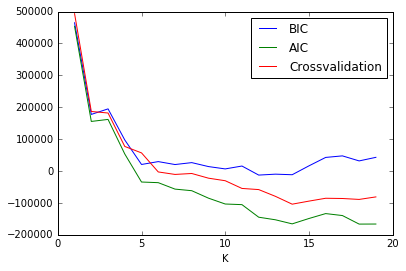
\includegraphics[width=0.7\textwidth]{Fig/BIC-AIC.png}
	\vspace{-5pt}
	\caption{BIC, AIC, and 10-fold crossvalidation}
	\label{fig:BIC-AIC}
\end{figure}

As it shown in fig.1, the group use BIC, AIC and 10-fold crossvalidation to assess the best number of clusters for the SPAM dataset. We compute the three measures for K = 1,...20, and use 10 replicates to avoid bad solutions due to poor initial conditions. Best result will be kepted. The model with lowest AIC and BIC value indicates the model with best trade-off. We can tell from fig.1 that when K = 5,both BIC and AIC reach a elbow, the distortion goes rapidly before that point. In this case, the group considers the ideal value of K would be 5.


We did a dimensionality reduction for the data before we did the cluster. The data has been reduced into two componets. The cluster of SPAM data by GMM with 5 clusters, is shown in fig.2.     

\vspace{-5pt}
%kommentar
\begin{figure}[!ht]
	\centering
	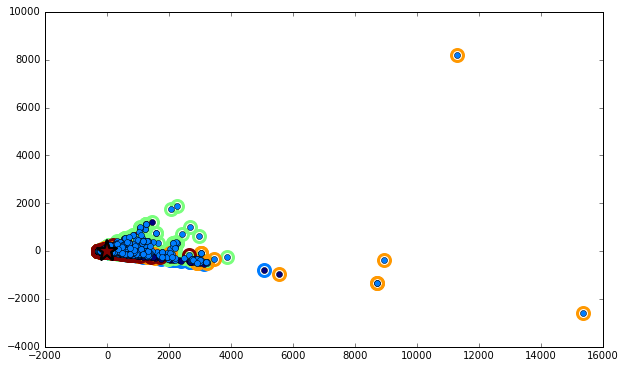
\includegraphics[width=0.7\textwidth]{Fig/GMM-plot.png}
	\vspace{-5pt}
	\caption{The cluster from GMM with 5 clusters}
	\label{fig:BIC-AIC}
\end{figure}
\newpage
\subsection{Hierarchical Clustering}
\newpage



